\documentclass[11pt,oneside,a4paper, german]{article}
\usepackage[german]{babel}
\usepackage[T1]{fontenc}
\usepackage{amsmath}
\usepackage{amsfonts}
\usepackage{mathtools}
\usepackage{amssymb}
\usepackage[utf8x]{inputenc}
\usepackage{enumerate}
\usepackage{graphicx}
%raender
\usepackage[textwidth=450pt]{geometry}
\title{Mathe II - Formelsammlung}
\author{Sallar Ahmadi-Pour}
\date{WiSe 2013/14}
\newcommand\numberthis{\addtocounter{equation}{1}\tag{\theequation}}


\DeclarePairedDelimiter\abs{\lvert}{\rvert}
\DeclarePairedDelimiter\norm{\lVert}{\rVert}

\addto\captionsgerman{\renewcommand*{\abstractname}{Vorwort}}
\begin{document}
\maketitle
\begin{abstract}
Diese Formelsammlung ist im Zuge der Veranstaltung 'Mathematik 2 - Analysis' des WiSe 2013/14 im Studiengang technische Informatik BSc. entstanden. Ich gewährleiste kein Vollständigkeit, Richtigkeit oder ähnliches. Jeder kann diese Formelsammlung nutzen. Ich stelle sie der Öffentlichkeit zur Verfügung und hoffe diese damit teilen zu können.
\end{abstract}
\tableofcontents
\section{Mengenlehre}

\subsection{Allgemeines}
\begin{align*}
M_E &= \{ a \enspace|\enspace a \text{ mit Eigenschaft } E\} &\text{Beschreibend}\\
M_A &= \{a_1 , a_2 , a_3 , \dots , a_n\} &\text{Aufzählend, abzählbar Endlich}\\
M &= \{a_1 , a_2 , a_3 , \dots \} &\text{abzählbar Unendlich}\\
M_AE &= \{ 1,2,3,\dots \} = \{n \enspace|\enspace n \in \mathbb{N} \} &\text{\underline{beides}}\\
a &\in M &\text{a Elemnt aus der Menge M}\\
a &\notin M &\text{a \underline{nicht} Element aus M}
\end{align*}

\subsection{Teilmenge} 
$A \subset B \to A$ Teilmenge von $B$ oder $B \supset A$. \\
$A = B$ wenn $A \subset B$ und $B \subset A$.
$$ x \in A \Leftrightarrow  x \in B $$

\subsection{Nullmenge} 
$M = \{ \} = \emptyset $

\subsection{Potenzmenge} 
Menge aller Teilmengen. \\
$A = \{1,2\}$ ; $P(A) = \{ \{1\},\{2\},\{1,2\},\emptyset \}$

\subsection{Anzahl der Elemente einer Menge} 
$\#A = |A| = 2$ und $|P(A)| = 4$.
$$|P(M)| = 2^{|M|}$$  

\subsection{Komplementärmenge}
Sei $A \subset M$, dann ist $\bar{A}$ die Komplementärmenge.\\
$\bar{A} = \{ x \enspace | \enspace x \in M \wedge x \notin A \}$\\
$\bar{M} = \emptyset$ und $\bar{\emptyset} = M$\\
$A \backslash M = \bar{A}$

\subsection{Vereinugungsmenge}
$A \cup B := \{ x \enspace | \enspace x \in A \vee x \in B \}$ \\
Man sagt auch: $A$ vereinigt $B$.

\subsection{Paarmenge / Produktmenge}
$A \times B := \{ (a,b) \enspace | \enspace a \in A, b \in B \}$\\
$A \cap B = \{ x \enspace | \enspace x \in A \wedge x \in B \}$\\
Man sagt auch $A$ und $B$.\\
Ist $B \subset A$ so heißt $A \backslash B$ Komplement $\bar{B}$ oder $B^c$.

\subsection{Rechenregeln}
Seien $A,B,C$ Mengen und $M$ das Einselement:
\begin{enumerate}[a)]
\item $A \cup B = B \cup A$ -- Kommutativ
\item $A \cap B = B \cap A$ -- Kommutativ
\item $(A \cup B) \cup C = A \cup ( B \cup C)$ -- Assoziativ
\item $(A \cap B) \cap C = A \cap ( B \cap C)$ -- Assoziativ
\item $A \cap (B \cup C) = (A \cap B) \cup (A \cap C)$ -- Distributiv
\item $A \cup (B \cap C) = (A \cup B) \cap (A \cup C)$ -- Distributiv
\item $A \cap (A \cup C) = A$ -- Verschmelzung
\item $B \cup (B \cap C) = B$ -- Verschmelzung
\item $A \cup \emptyset = A$ aber $A \cap \emptyset = \emptyset$
\item $A \cap M = A$ aber $A \cup M = M$
\item $A \cup \bar{A}$ und $A \cap \bar{A} = \emptyset$ -- Komplement-Eigenschaft
\item $\bar{\bar{A}} = A$
\item $\overline{A \cup B} = \bar{A} \cap \bar{B}$ -- DeMorgansche Regel
\item $\overline{A \cap B} = \bar{A} \cup \bar{B}$ -- DeMorgansche Regel
\end{enumerate}

\subsection{Abbildungen}
Eine Abbildung ist {\sc surjektiv}: $\forall b \in B \exists a \in A, f(a) = b$.\\
Eine Abbildung ist {\sc injektiv}: $\forall a,a' \in A a\neq a' \Rightarrow f(a) \neq f(a')$.\\
Eine Abbildung ist {\sc bijektiv} wenn sie surjektiv und injektiv ist.

\subsection{Anzahl der Elemente einer unendlichen Menge}
\paragraph{abzählbare Unendlichkeit} Sei $M$ eine Menge. $M$ heißt  unendlich, falls es eine echte Teilmenge $N\subset M$ gibt, die sich bijektiv auf $M$ abbilden lässt. Eine Menge heißt endlich, wenn sie nicht unendlich ist.
\paragraph{Abzählbarkeit} Eine Menge heißt abzählbar unendlich, wenn eine Bijektion zwischen $M$ und $N$ existiert. $|\mathbb{N}| = \infty$

\section{Vollständige Induktion}
\subsection{Allgemeines}
Ein Beweis mit vollständiger Induktion (z.B. einer Summenformel bzw. deren nicht iterativer Formel) besteht immer aus:

\begin{enumerate}[$\bullet$]
\item \underline{Induktionsbehauptung}: hier wird die zu beweisende Gleichung niedergeschrieben. Dies ist unsere Induktionsannahme.
\item Dann folgt der \underline{Induktionsanfang}, hier wird ein (möglichst einfacher) Fall -- für z.B. $n=1$ durchgerechnet.
\item Sollte der Induktionsanfang korrekt sein, kann man nun den \underline{Induktionsschritt} vollziehen. Hierbei muss die Induktionsbehauptung verwendet werden. Durch geschicktes Umformen gelangt man nun zu einer aussage, welcher für n+1 gilt. Somit sei eine Behauptung mit vollständiger Induktion bewiesen.
\item Als letztes kommt der \underline{Induktionsschluss}. Hier wird die Formel erneut niedergeschrieben, jedoch mit zugehörigem Definitionsbereich (z.B. für alle $n \geq 1$).
\end{enumerate}

\subsection{Beispiele}
Sei $\sum_{k=1}^{n} \frac{k}{2^k} = 2 - \frac{n+2}{2^n}$ unsere Induktionsbehauptung welche zu beweisen gilt, so folgt daraus:
\begin{align*}
\sum_{k=1}^{n} \frac{k}{2^k} &= 2 - \frac{n+2}{2^n} \numberthis \label{eqn:IB} \\ 
\sum_{k=1}^{1} \frac{k}{2^k} &= 2 - \frac{1+2}{2^1} \numberthis \label{eqn:IA} \\ 
\intertext{für alle $n\geq 1$ sei die Behauptung richtig}\\
\sum_{k=1}^{n+1} \frac{k}{2^k} &= \sum_{k=1}^{1} \frac{k}{2^k} + \frac{n+1}{2^{n+1}} \numberthis \label{eqn:ISt} \\ 
&= 2 - \frac{n+2}{2^n} + \frac{n+1}{2^n} \\ 
&= 2 + \frac{-n-2}{2^n} + \frac{n+1}{2^{n+1}} \\ 
&= 2 + \frac{-2n-4 + n+1}{2^{n+1}} \\ 
&= 2+ \frac{-n-3}{2^{n+1}} \\ 
&= 2 - \frac{n+3}{2^{n+1}} \\ 
&= 2- \frac{(n+1)+2}{2^{n+1}}\\
\sum_{k=1}^{n} \frac{k}{2^k} &= 2 - \frac{n+2}{2^n} \text{\quad gilt für alle $n\geq 1$.} \numberthis \label{eqn:ISch}
\end{align*}
Bei diesem Beispiel ist Gleichung \eqref{eqn:IB} die Induktionsbehauptung bzw. -annahme, \eqref{eqn:IA} der Induktionsanfang, \eqref{eqn:ISt} der Induktionsschritt mit Umformung und \eqref{eqn:ISch} der Induktionsschluss.
\\
Sei $2^n < n!$ unsere Induktionsbehauptung welche zu beweisen gilt, so folgt daraus:
\begin{align*}
2^{n_0} &< n_0! \\
2^4 = 16 &< 4! = 24 \\
\intertext{für $n\geq 4$ sei $2^n < n!$}\\
n &\rightarrow n+1\\
2^n &< n! \text{\quad gilt $\forall n \geq 4$}
\end{align*}
\include{gruppe_ring}
\include{komplexe}
\section{Abbildungen und Funktionen}
\subsection{Grundbegriffe}
Eine Abbildung $f: A \rightarrow B$ heißt Funktion von A nach B, wenn jedem $a \in A$ genau ein $b \in B$ zugeordnet wird. $b = f(a)$ heißt Funktionswert an der Stelle $a$. Der Definitionsbereich $\mathbb{D}$ sind die Werte,  die in die Funktion als $a$ eingegeben werden können. Der Wertebereich $\mathbb{W}$ sind die Werte, die aus der Funktion resultieren. Die Bereiche können als übliche Mengen mit Eigenschaft niedergeschrieben werden z.B. :
\begin{align*}
\mathbb{D}(f(x)) &= \{ x \in \mathbb{R} \enspace | \enspace x \}\\
\mathbb{W}(f(x)) &= \{ y \in \mathbb{R} \enspace | \enspace y \}
\end{align*}
\subsection{Gerade und ungerade Funktion}
\begin{align*}
f(-x) &= f(x) &\text{Gerade Funktion}\\ 
f(-x) &= -f(x) &\text{Ungerade Funktion}
\end{align*}
\subsection{Periodische Funktionen}
\begin{align*}
f(x+\lambda ) = f(x)
\end{align*}
Kleinstes $\lambda > 0$ ist die \underline{primitive Periode}.
\subsubsection{Beschränktheit}
Es sei $f: A \rightarrow B$. $M \subset A$ beschränkt an $K$.\\
Beispiel: $f(x) = \sin{x}$
$$| \sin{x} | \leq 1 \quad \forall x \in \mathbb{R}$$
Kleinste obere Schranke einer Funktion heißt \underline{Supremum}.
\begin{align*}
f(x) &= \sin{x}\\
\sup{f} &= 1
\end{align*}
Größte untere Schranke heißt \underline{Infimum}.
\begin{align*}
\inf{f} &= -1
\end{align*}
\subsubsection{Monotonieverhalten}
Eine Funktion $f: A \rightarrow B$ heißt im Intervall $I \subset A$ monoton wachsend bzw. streng monoton wachsend, wenn $\forall x_1,x_2 \in I$ mit $x_1 > x_2$ die Ungleichung 
$$f(x_1) \geq f(x_2) \quad \text{bzw.} \quad f(x_1) > f(x_2)$$
gilt. Entsprechend heißt sie monoton fallend bzw. streng monoton fallend, wenn $\forall x_1,x_2 \in I$ mit $x_1 > x_2$ die Ungleichung
$$f(x_1) \leq f(x_2) \quad \text{bzw.} \quad f(x_1) < f(x_2)$$
\subsection{Elementare Funktionen}
\subsubsection{Polynome}
Ein Polynom ist definiert durch:
$$f(x) = a_0 + a_1 x + \cdots + a_n x^n = \sum_{k=0}^n a_k x^k$$
Addition/Subtraktion:
$$\sum_{k=0}^n a_k x^k \pm \sum_{k=0}^n b_k x^k = \sum_{k=0}^n (a_k \pm b_k) x^k$$
Multiplikation:
$$\sum_{k=0}^n a_k x^k \cdot \sum_{k=0}^n b_k x^k = \sum_{k=0}^n a_k x^k \cdot \sum_{l=0}^n b_l x^l = \sum_{k=0}^n \sum_{l=0}^n a_k b_l x^{k+l}$$
\subsubsection{Lineare Funktion}
Die Hauptform der linearen Funktion lautet $f(x) = a_0 + a_1 x$. $a_0$ und $a_1$ können mit zwei Wertepaaren von $f(x)$ bestimmt werden:
\begin{align*}
a_1 &= \frac{y_2 - y_1}{x_2 - x_1}\\
a_0 &= y_1 - \frac{y_2 - y_1}{x_2 - x_1}x_1 = \frac{y_1 x_2 - y_2 x_1}{x_2 - x_1}
\end{align*}
Die Zweipunktform der linearen Funktion lautet $\frac{y - y_1}{x - x_1} = \frac{y_2 - y_1}{x_2 - x_1}$.\\
Die Achsenabschnittsform lautet $\frac{x}{a} + \frac{y}{b} = 1$. Mit $f(0) = b$ und $f(a)=0$.
\subsubsection{Quadratische Funktion}
Die Hauptform der quadratischen Funktion lautet $f(x) = a_0 + a_1 x + a_2 x^2$.\\
Die Nullstellen der quadratischen Funktion lassen sich über die p,q-Formel bestimmen. Diese leitet sich aus der Hauptform her:
\begin{align*}
a_2 x^2 + a_1 x + a_0 &= 0 &:a_2\\
x^2 + p x + q &= 0 &\text{mit $p = \frac{a_1}{a_2}, q = \frac{a_0}{a_2}$}\\
\Rightarrow x_{1/2} &= - \frac{p}{2} \pm \sqrt{(\frac{p}{2})^2 - q} &\text{p,q-Formel}
\end{align*}
Die Nullstellen lassen sich ebenfalls mithilfe der Mitternachtsformel bestimmen:
\begin{align*}
x_{1/2} &= \frac{-b \pm \sqrt{b^2 - 4ac}}{2a}\\
\text{Diskriminante} \quad D &= b^2 - 4ac\\
\end{align*}
Dabei gelten für die Diskriminante $D$ folgende Eigenschaften und Folgen für die Funktion:
\begin{tabular}{c l}
$D>0$ & reelle Lösung $x_1 | x_2$ \\
$D=0$ & eine doppelte reelle Lösung\\
$D<0$ & zwei Lösungen in $\mathbb{C}$ die konjugiert-komplex zueinander sind\\
\end{tabular}
\paragraph{Wurzelsatz von Vi\"{e}ta} ist für $\mathbb{C}$ als auch $\mathbb{R}$ gültig und lautet:
\begin{align*}
p &= -(x_1 + x_2)\\
q &= x_1 \cdot x_2
\end{align*}
\paragraph{Das Horner-Schema} erlaubt es in wenigen Rechenschritten Nullstellen als auch Funktionswerte zu berechnen. Diese Methode erweist sich als einfach für Computerprogramme zu implementieren. Außerdem erlaubt es die Berechnung von Funktionswerten ohne Taschenrechner\footnote{ Als Beispiel:
$11 + 7x - 5x^2 -4x^3 + 2x^4 \;=\; 11 + x \cdot\left(7 + x \cdot(-5 + x \cdot(-4 + x \cdot 2))\right)$}\\
Beispiel: $f(x) = 5x^6 - 2x^5 + 2x^3 + x^2 - 6x +1$. Zur Berechnung vom Funktionswert $f(2)$ sieht das Horner-Schema wie folgt aus:\\

\begin{figure}[!ht]
\caption{Horner-Schema für $f(x)$}
\centering
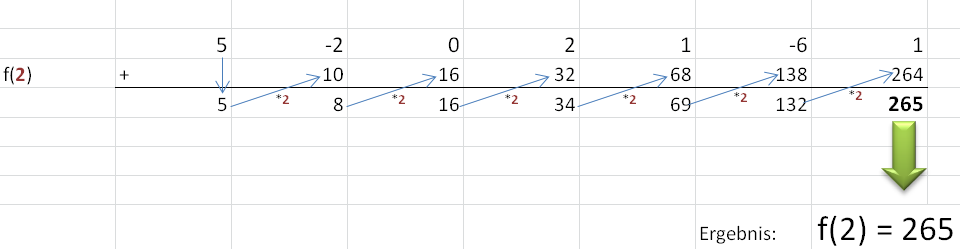
\includegraphics[scale=0.55]{img/img1}
\end{figure}


\include{gebrochen}
\subsection{Exponential- und Logartihmusfunktion}
Die Exponentialfunktion ist eine Abbildung $f: \mathbb{R} \rightarrow \mathbb{R}$ mit 
$$f(x) = e^x = \exp{(x)} := \lim_{n\rightarrow \infty}(1+\frac{x}{n})^n , x\in \mathbb{R}$$
Alternativ ist auch folgendes möglich: $e^x := \sum^{\infty}_{n=0} \frac{x^n}{n!}$.\\
Für die Exponentialfunktion gelten alle Potenzgesetze. \\
$f(x) = e^x \Rightarrow f(x) < 0 \quad \forall x \in \mathbb{R}$. $e^x$ ist streng monoton wachsend $\Rightarrow$ $e^x$ ist injektiv. $f: \mathbb{R} \rightarrow (0,\infty)$ ist bijektiv.\\
Die Umkehrfunktion der Exponentialfunktion ist die Logarithmusfunktion. Im Fall von $e^x$ ist $f^-1(x)$ der logarithmus Naturalis (der Logarithmus zur Basis $e$) $\log_e{x} = \ln(x)$. Für den natürlichen Logarithmus gelten alle Logarithmusregeln.
\include{trig_fkt}
\end{document}
